\SourcePage{375}{378}
\section{Valence}

The capacity of atoms to join together into a molecule is described through the notion of \emph{valence}. A definite valence is assigned to each atom, and when atoms combine, their valences must saturate one another: every valence bond of one atom must be matched by a valence bond of another. Thus, in the methane molecule $\mathrm{CH}_4$, the four bonds of tetravalent carbon are saturated by bonds from four monovalent hydrogen atoms. To give valence a physical interpretation, we begin with the simplest case, in which two hydrogen atoms unite to form an $\mathrm H_2$ molecule.

Consider two hydrogen atoms in their ground states (${}^2S$). When brought near each other, they can form a system in either the ${}^1\Sigma_g^+$ or the ${}^3\Sigma_u^+$ molecular state. The singlet term has an antisymmetric spin wave function, while the triplet term has a symmetric one. For the coordinate wave function the symmetry is reversed: it is symmetric for the ${}^1\Sigma$ term and antisymmetric for the ${}^3\Sigma$ term. It is plain that only ${}^1\Sigma$ can be the ground term of the $\mathrm H_2$ molecule. Indeed, an antisymmetric wave function $\psi(\mathbf r_1,\mathbf r_2)$ (where $\mathbf r_1$ and $\mathbf r_2$ are the radius vectors of the two electrons) necessarily has nodes---it vanishes when $\mathbf r_1=\mathbf r_2$---and therefore cannot describe the lowest state of the system.

Numerical calculation confirms that the ${}^1\Sigma$ electronic term has a pronounced minimum, corresponding to the formation of a stable $\mathrm H_2$ molecule. In the ${}^3\Sigma$ state, by contrast, the energy $U(r)$ decreases monotonically as the distance between the nuclei increases; this describes mutual repulsion of the two H atoms\footnote{Here we disregard the van der Waals attraction between the atoms (see \S~89). Its existence means that the $U(r)$ curve for the ${}^3\Sigma$ term also has a minimum, situated at large distances. This minimum, however, is very shallow relative to that on the ${}^1\Sigma$ curve and would be invisible on the scale of Fig.~29.} (Fig.~29).

\SourcePage{376}{379}
Thus the total spin of a hydrogen molecule in its ground state is zero, $S=0$. The molecules of virtually all chemically stable compounds of the main-group elements prove to have this property. Among inorganic molecules, the exceptions are the diatomic molecules $\mathrm O_2$ (ground state ${}^3\Sigma$) and NO (ground state ${}^2\Pi$), as well as the triatomic molecules $\mathrm{NO}_2$ and $\mathrm{ClO}_2$ (total spin $S=1/2$). The transition-group elements have special features; these will be considered below, after the valence properties of the main-group elements have been examined.

\begin{figure}[ht]
\centering
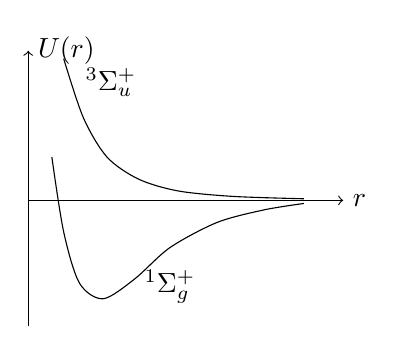
\begin{tikzpicture}[x=1cm,y=1cm]
 \draw[->] (0,-1.6)--(0,1.9) node[right] {$U(r)$};
 \draw[->] (0,0)--(4,0) node[right] {$r$};
 \draw[smooth] plot coordinates {(.45,1.8)(.7,1.05)(1.0,.55)(1.4,.27)(1.9,.12)(2.6,.05)(3.5,.02)};
 \draw[smooth] plot coordinates {(.3,.55)(.45,-.4)(.65,-1.05)(.95,-1.25)(1.35,-1.0)(1.8,-.6)(2.4,-.28)(3.0,-.12)(3.5,-.04)};
 \node at (1.05,1.5) {$^3\Sigma_u^+$};
 \node at (1.8,-1.1) {$^1\Sigma_g^+$};
\end{tikzpicture}
\caption*{Fig. 29}
\end{figure}

The ability of atoms to unite is therefore connected with their spin (W.~Heitler, H.~London, 1927). Combination occurs in such a way that the atomic spins compensate one another. A convenient quantitative measure of an atom's ability to combine is the integer twice its spin. This number is the same as the atom's chemical valence. One must remember here that a given atom can have different valences according to the state in which it is found.

Let us apply this viewpoint to the main groups of the periodic system. In the normal state, first-group elements (the first column of Table~3, the alkali-metal group) have spin $S=1/2$ and hence valence one. A state of higher spin could be produced only by exciting an electron out of a filled shell. Such states lie so high that an excited atom cannot form a stable molecule\footnote{For the elements Cu, Ag, and Au, see the end of this section.}.

In the normal state, atoms of the second-group elements (the second column of Table~3, the alkaline-earth-metal group) have $S=0$. These atoms therefore cannot enter chemical compounds while in their normal state. Fairly near the ground state, however, there is
\SourcePage{377}{380}
an excited state whose unfilled shell has configuration $sp$ instead of $s^2$ and whose total spin is $S=1$. In this state the atom has valence 2, which is the principal valence of second-group elements.

The normal-state configuration of third-group elements is $s^2p$, with spin $S=1/2$. Excitation of an electron from the filled $s$ shell, however, produces a nearby excited state of configuration $sp^2$ and spin $S=3/2$. Elements of this group accordingly display both monovalent and trivalent behavior. The first elements of the group (B, Al) behave only as trivalent elements. The tendency to exhibit valence 1 becomes stronger with increasing atomic number, and Tl behaves to the same extent as a monovalent and as a trivalent element (for example, in TlCl and $\mathrm{TlCl}_3$). The reason is that, for the early elements of the group, the energetic advantage from the greater bond energy in compounds of the trivalent element, relative to those of the monovalent element, outweighs the atomic excitation energy.

For fourth-group atoms the ground state has configuration $s^2p^2$ and spin 1, while a nearby excited state has configuration $sp^3$ and spin 2. The respective valences are 2 and 4. As in the third group, the first members of the fourth group (C, Si) chiefly exhibit the higher valence (CO, for example, is an exception), whereas the propensity for the lower valence increases with atomic number.

In atoms of the fifth group, the ground state has configuration $s^2p^3$ and spin $S=3/2$, giving valence three. A higher-spin excited state can arise only when one of the electrons passes to a shell with the next principal quantum number. The nearest state of this kind has configuration $sp^3s'$ and spin $S=5/2$ (here $s'$ conventionally denotes an electron $s$ state whose principal quantum number is one greater than that of the $s$ state). Although the excitation energy of this state is comparatively large, the excited atom can nevertheless enter a stable compound. Fifth-group elements consequently occur as both trivalent and pentavalent elements (nitrogen, for instance, is trivalent in $\mathrm{NH}_3$ and pentavalent in $\mathrm{HNO}_3$).

For sixth-group elements the ground-state configuration is $s^2p^4$ and the spin is 1, so the atom is divalent. Exciting one $p$ electron gives the state $s^2p^3s'$ with spin 2; excitation of one more $s$ electron gives the state
\SourcePage{378}{381}
$sp^3s'p'$ with spin 3. In either excited state, the atom can become part of a stable molecule and displays valence 4 or 6, respectively. The first element of the sixth group (oxygen) has only valence 2, whereas later members also show the higher valences (thus sulfur is respectively divalent, tetravalent, and hexavalent in $\mathrm H_2S$, $\mathrm{SO}_2$, and $\mathrm{SO}_3$).

In the seventh group (the halogens), atoms in the ground state (configuration $s^2p^5$, spin $S=1/2$) are monovalent. They can, however, also form stable compounds in excited states of configurations $s^2p^4s'$, $s^2p^3s'p'$, and $sp^3s'p'^2$, having spins $3/2$, $5/2$, and $7/2$, respectively; these correspond to valences 3, 5, and 7. The first element of the group (F) is invariably monovalent, while later members also display the higher valences (chlorine, for example, is respectively mono-, tri-, penta-, and heptavalent in HCl, $\mathrm{HClO}_2$, $\mathrm{HClO}_3$, and $\mathrm{HClO}_4$).

Finally, atoms of the noble-gas elements have completely filled shells in their ground state. Their spin is therefore $S=0$, and their excitation energies are large. Accordingly, their valence is zero, and these elements are chemically inert.
\unskip
\footnote{A few of them nevertheless form stable compounds, for example with fluorine or oxygen. Such valences may arise when electrons are promoted out of the filled outer shell. The electrons then enter unoccupied $f$- (or $d$-) states lying relatively close in energy.

We should also note a distinctive attraction. It appears when a noble-gas atom interacts with an excited atom of the same element. Two identical atoms are then brought together while occupying different states. The number of possible states produced in this way is doubled (see \S~80). Transfer of the excitation from one atom to the other takes the place of the exchange interaction that produces ordinary valence. The molecule $\mathrm{He}_2$ provides an example. Bonding of the same kind occurs in molecular ions made up of two identical atoms. One example is $\mathrm H_2^+$.}


All these arguments call for the following general qualification. To say that an atom enters a molecule with the valence belonging to one of its excited states does not imply that separating the atoms to large distances must yield an excited atom. It means only that the molecular electron-density distribution near the nucleus of the atom in question resembles that in an isolated excited atom. Yet the limiting electron distribution reached as the internuclear distance grows may correspond to unexcited atoms.

\SourcePage{379}{382}
When atoms form a molecule, their filled electron shells change little. The distribution of electron density in unfilled shells, on the other hand, can change substantially. In the most pronounced cases of a so-called \emph{heteropolar bond}, all valence electrons pass from some atoms to others. The molecule may then be said to consist of ions whose charges, in units of $e$, are equal to their valences. The first-group elements are electropositive: in heteropolar compounds they give up electrons and form positive ions. Across the subsequent groups electropositivity gradually diminishes and gives way to electronegativity, which is strongest among the seventh-group elements. The same qualification made above for excited atoms in molecules must also be applied to heteropolarity. A heteropolar molecule need not necessarily yield two ions when its atoms are separated. Thus, separation of CsF would indeed give $\mathrm{Cs}^+$ and $\mathrm F^-$ ions, but NaF tends instead to neutral Na and F atoms (because fluorine's electron affinity exceeds the ionization potential of cesium but is below that of sodium).

At the opposite limit is the so-called \emph{homopolar bond}. The atoms in such a molecule remain neutral on average. Unlike heteropolar molecules, homopolar molecules possess no appreciable dipole moment. The distinction between heteropolar and homopolar bonding is entirely quantitative, and every intermediate case is possible.


We now turn to the transition-group elements. In the character of their valence properties, the elements of the palladium and platinum groups differ little from main-group elements. The distinction is that their $d$ electrons lie comparatively deep in the atom and therefore interact more weakly with other atoms in a molecule. As a result, ``unsaturated'' compounds, whose molecules have nonzero spin (in fact no greater than $1/2$), are encountered relatively often among compounds of these elements. Each element can show several valences, and here they may differ by one rather than only by two as in main-group elements (where a change of valence is tied to the excitation of an electron whose spin was compensated, thereby freeing the spins of a pair of electrons at once).

Rare-earth elements are characterized by an unfilled $f$ shell. The $f$ electrons lie much
\SourcePage{380}{383}
deeper than the $d$ electrons and consequently take no part at all in valence. Thus only $s$ and $p$ electrons in unfilled shells determine the valence of rare-earth elements\footnote{The $d$ electrons present in unfilled shells of the atoms of some rare-earth elements are immaterial, since in practice these atoms always enter compounds in excited states containing no $d$ electrons.}. It should be borne in mind, however, that atomic excitation can transfer $f$ electrons into $s$ and $p$ states and thereby increase the valence by one. Rare-earth elements therefore also show valences differing by one (in practice, they are all tri- and tetravalent).

The elements of the actinium group occupy a special position. Ac and Th contain no $f$ electrons at all, and their $d$ electrons participate in valence; their chemical properties therefore resemble those of the palladium and platinum groups rather than those of the rare earths. Although a U atom contains $f$ electrons in its normal state, uranium likewise has no $f$ electrons in its compounds. Finally, atoms of Np, Pu, Am, and Cm retain $f$ electrons even in compounds, but for them too it is the $s$ and $d$ electrons that participate in valence. In this sense they are homologues of uranium. The greatest possible numbers of ``unpaired'' $s$ and $d$ electrons are 1 and 5, respectively; hence the maximum valence of actinium-group elements is six (whereas the maximum for rare-earth elements, with $s$ and $p$ electrons participating in valence, is $1+3=4$).

With respect to valence properties, the iron-group elements stand between the rare-earth elements and those of the palladium and platinum groups. In their atoms the $d$ electrons lie relatively deep and, in many compounds, take no part at all in the valence bond. In these compounds, therefore, the iron-group elements behave like rare-earth elements. These include ionic compounds (for example, $\mathrm{FeCl}_2$ and $\mathrm{FeCl}_3$), in which the metal atom enters as a simple cation. As with the rare earths, iron-group elements can display many different valences in compounds of this type.

Another class of compounds formed by the iron-group elements consists of the so-called complex compounds.
Their distinguishing feature is that the transition-element atom does not enter the molecule as a simple ion.
Instead, it forms part of a composite, or complex, ion.
One example is the ion $\mathrm{MnO}_4^-$ in $\mathrm{KMnO}_4$.
Another is the ion $\mathrm{Fe(CN)}_6^{4-}$ in $\mathrm K_4Fe(CN)_6$.
In such complex ions the atoms

\SourcePage{381}{384}
lie closer together than in simple ionic compounds, and their $d$-electrons take part in valence bonding.
Accordingly, in complex compounds the iron-group elements behave like the elements of the palladium and platinum groups.


Finally, a qualification is needed concerning Cu, Ag, and Au, which were placed among the main groups in \S~73: in a number of compounds they behave as transition elements. They can exhibit valence greater than one by transfer of electrons from the $d$ shell to the energetically nearby $p$ shell (for example, from $3d$ to $4p$ in Cu). In these compounds the atoms have an unfilled $d$ shell and behave as transition elements (Cu like an iron-group element, and Ag and Au like palladium- and platinum-group elements).

\ProblemHeading Determine the electronic terms of the molecular ion $\mathrm H_2^+$ formed by combining a hydrogen atom in its normal state with an $\mathrm H^+$ ion, when the distance $R$ between the nuclei is large compared with the Bohr radius (L.~D.~Landau, 1961; C.~Herring, 1961)\footnote{For the solution of the analogous problem for the $\mathrm H_2$ molecule, see L.~P.~Gor'kov, L.~P.~Pitaevskii~// Dokl. Akad. Nauk SSSR. 1963. Vol.~151. P.~822; C.~Herring, M.~Flicker~// Phys. Rev. 1964. Vol.~134A. P.~362 (the computational error made in the first paper is corrected in the second).}.

\SolutionHeading In its formulation this problem is analogous to Problem~3 of \S~50. Instead of two one-dimensional potential wells, there are now two three-dimensional wells (around the two nuclei), with a common axial symmetry about the line joining the nuclei. The level $E_0=-1/2$ (the ground level of the hydrogen atom)\footnote{Atomic units are used in this problem.} splits into levels $U_g(R)$ and $U_u(R)$ (the ${}^2\Sigma_g^+$ and ${}^2\Sigma_u^+$ terms), corresponding to the electron wave functions
\[\psi_{g,u}(x,y,z)=\frac1{\sqrt2}[\psi_0(x,y,z)\pm\psi_0(-x,y,z)],\]
which are respectively symmetric and antisymmetric with respect to the plane $x=0$ bisecting the distance between the nuclei (located at $x=\pm R/2$ on the $x$ axis). Here $\psi_0(x,y,z)$ is the electron wave function in one of the potential wells. Proceeding exactly as in Problem~3 of \S~50 gives
\begin{equation}U_{g,u}(R)-E_0=\mp\int\psi_0\frac{\partial\psi_0}{\partial x}\,dy\,dz,\tag{1}\end{equation}
where the integration extends over the plane $x=0$\footnote{Thus the effect being sought is determined by the range of distances in which the electron interacts equally with the two nuclei.}.

\SourcePage{382}{385}
We seek the function $\psi_0$ (for motion, say, about nucleus 1 at $x=R/2$) in the form
\begin{equation}\psi_0=\frac1{\sqrt\pi}e^{-r_1}a,\tag{2}\end{equation}
where $a$ varies slowly (for a hydrogen atom, $a$ would be 1). The function $\psi_0$ must satisfy the Schrödinger equation
\begin{equation}\frac12\Delta\psi_0+\left(-\frac12-\frac1R+\frac1{r_1}+\frac1{r_2}\right)\psi_0=0\tag{3}\end{equation}
($r_1$ and $r_2$ are the electron's distances from nuclei 1 and 2). The electron's total energy appearing in this equation is the difference $E_0-1/R$, since $E_0$ itself also includes the energy $1/R$ of Coulomb repulsion between the nuclei.

Since $\psi_0$ decreases rapidly away from the $x$ axis, only values of $y,z$ small compared with $R$ contribute appreciably to the integral (1). For $y,z\ll R$, substitution of (2) in (3) yields
\[\frac{\partial a}{\partial x}+\frac{R/2+x}{R}a=0\]
(second derivatives of the slowly varying function $a$ have been neglected, and $r_2$ has been set equal to $R/2+x$). The solution that tends to unity as $x\to R/2$ (that is, near nucleus 1) is
\[a=\frac{2R}{R+2x}\exp\left(\frac{x}{R}-\frac12\right).\]
Formula (1) now gives
\[U_{g,u}-E_0=\mp\frac4e\int_{R/2}^{\infty}e^{-2r_1}2\pi r_1,dr_1=\mp2Re^{-R-1}.\]
The splitting is therefore\footnote{The analogous result for the $\mathrm H_2$ molecule (see the papers cited above) is $U_g-U_u=-1{,}64R^{5/2}e^{-2R}$.}
\begin{equation}U_g-U_u=-4Re^{-R-1}.\tag{4}\end{equation}

At sufficiently large distances this exponentially decreasing expression becomes smaller than the second-order effect of the dipole interaction between the H atom and the $\mathrm H^+$ ion. The polarizability of a hydrogen atom in its normal state is $9/2$ (see (77.9)), and the field of the $\mathrm H^+$ ion is $\mathcal E=1/R^2$; the corresponding interaction energy is consequently $-9/(4R^4)$. Including it gives
\begin{equation}U_{g,u}(R)-E_0=\mp2Re^{-R-1}-\frac9{4R^4}.\tag{5}\end{equation}
The second term becomes comparable to the first only at $R=10.8$.
The term $U_u(R)$ also possesses a minimum.
It lies at $R=12.6$.
Its value is $-5.8\cdot10^{-5}$ atomic units ($-1.6\cdot10^{-3}$ eV)\footnote{This minimum, arising from van der Waals forces, is very shallow in comparison with the minimum of the term $U_g(R)$, which corresponds to the normal state of the stable ion $\mathrm H_2^+$; that principal minimum lies at $R=2.0$ and equals $-0.60$ atomic units ($-16.3$ eV).}.

